% !TeX spellcheck = en_GB
\chapter{Load balancing}

When dealing with redundant distributed systems, there exists more than one node capable of doing some work.
In such a system the workload needs to be distributed and balanced across all nodes.
This is done using a load balancer with a node balancing algorithm and some performance optimising features.

A node balancer is the 

%icons from http://www.cisco.com/web/about/ac50/ac47/2.html
\begin{tikzpicture}[
	start chain=going right,
	diagram item/.style={
		minimum width=90pt,
%		minimum height=45pt,
		on chain,
		join
	}
]
\node [
	diagram item,
  label=center:Internet
] {
\includegraphics{Cisco_BW/cloud}};

\node [
	continue chain=going below,
	diagram item,
	label=right:Router
] {
\includegraphics{Cisco_BW/router}};

\node [
	start branch=1 going below right,
	diagram item,
	label=right:Load Balancer 2
] (LB2) {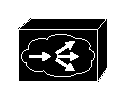
\includegraphics{Cisco_BW/distributed_director}};

\node [
	continue chain=going below left,
	diagram item,
	label=right:Load Balancer 1
] {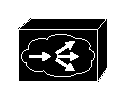
\includegraphics{Cisco_BW/distributed_director}};

\node [
	continue chain = going below right,
	diagram item,
	label=right:Services in the distrinbuted in teh farm
] (farm) {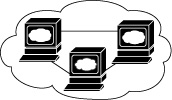
\includegraphics{Cisco_BW/web_cluster}};

\draw (LB2) -> (farm);

\node [
	start branch=1 going below right,
	diagram item,
	label=below:Http interface
] {\includegraphics{Cisco_BW/PC}};

\node [
	start branch=1 going below left,
	diagram item,
	label=below:OPC XML interface
] {\includegraphics{Cisco_BW/PC}};


\node [
	continue chain = going below,
	diagram item,
	label=below:mod Bus interface
] {\includegraphics{Cisco_BW/PC}};


\end{tikzpicture}

In this solution the load balancer needs to balance external connections to different protocols like HTTP and Modbus, however a solution witch can be extended to any restful protocol is needed. Also balancing of node roles depending on the amount incoming traffic on different interfaces will be needed.

Load balancers can also provide different features like bundling requests, security, discovering bad nodes and caching (Squid). This can offload the servers behind.

The following requirements to the system exists:
\begin{description}
	\item Robustness
	\item Protocol flexible
	\item support TCP Handoffs (for non restful applications)
	\item Must be a distributed component
\end{description}

\section{Levels of balancing}
\begin{description}
	\item[OSI 3] Network/IP %google says network layer LVS says transport layer
	\item[OSI 4] Network/IP
	\item[OSI 7] {Application level, like http balancing, allows balancing strategies based on url and user location.}
\end{description}

What we would like is a transport layer protocol.
\cite{Ludwig:SwarmIntelligenceGridLoadBalancing} Implements a particle swam based algorithm, and discuses quality parameters.

\section{Existing solutions}
\begin{description}
	\item[Linux Virtual Server: IPVS] Is implemented in the linux kernal version 2.4 and 2.6. Works at the IP level. Useed byt big sites sourceforge.net, layer 3.
	\item[Google Compute Engine: Load Balancer]: Proprietary. layer 3 and 7.
\end{description}